\documentclass[../main.tex]{subfiles}

% 2.2.1 Wellenverhalten bei Substanzen
Beim zusammenkommen einer Welle mit einer Substanz kann es zu verschiedenen Abschwächungen der Welle kommen. Es spielen Absorption, Streuung, Beugung und Reflexion (Abb. \ref{fig:extinktion_typen}) eine Rolle.

% TODO alternative image (copyright..)
\begin{figure}[ht]
    \centering
    \includegraphics[width=0.65\textwidth]{extinktion_typen.png}
    \caption{Einflussfaktoren auf Extinktion}
    \label{fig:extinktion_typen}
\end{figure}

% 2.2.2 Streuung
\textbf{Streuung} ist die Ablenkung von Wellen in mehrere Richtungen.
% 2.2.3 Beugung
Wenn Strahlungen eine Substanz mit unterschiedlicher Dichte durchqueren, kommt es zu einer Verlangsamung der Ausbreitung, und damit zu einer Richtungsänderung - das ist \textbf{Beugung}.
% 2.2.4 Reflexion
Glatte Oberflächen \textbf{reflektieren} häufig Strahlungen (z.B. Spiegel).

% 2.2.5 Absorption
\textbf{Absorption} beschreibt in der Physik die Aufnahme von Wellen in einer Substanz. Diese ist für die IR-Spektroskopie besonders interresant, da beim Zusammenkommen von Infrarotlicht mit einer Substanz Vibrationsmuster in den Molekülen auftreten, anhand dessen sich der Aufbau der Substanz ableiten lassen kann. Verschiedene funktionelle Gruppen in der Chemie haben nämlich bei verschiedenen Wellenlängen Absorptionseigenschaften. So treten z.B. bei Wasser ($H_2O$) Absorptionen bei \SI{2.734}{\micro\metre}, \SI{6.269}{\micro\metre} und \SI{2.662}{\micro\metre} auf. Die Vibrationsmuster sind jeweilig symmetrisches Dehnen der $OH$-Bindungen (Abb. \ref{fig:oh_symmetric_stretching}), $H-O-H$-Beugung (Abb. \ref{fig:hoh_bending}) und $OH$-asymetrisches Dehnen (Abb. \ref{fig:oh_asymmetric_stretching}).

\begin{figure}
    \centering
    \begin{subfigure}[b]{0.3\textwidth}
        \chemfig{
            O(-[:135,0.8]H)(-[:45,0.8]H)
        }
        \hspace{0.1cm}
        \chemfig{
            O(-[:135,1.2]H)(-[:45,1.2]H)
        }
        \caption{OH Symmetrisches Dehnen}
        \label{fig:oh_symmetric_stretching}
    \end{subfigure}
    \begin{subfigure}[b]{0.3\textwidth}
        \chemfig{
            O(-[:135]H)(-[:45]H)
        }
        \hspace{0.1cm}
        \chemfig{
            O(-[:160]H)(-[:20]H)
        }
        \caption{HOH Beugung}
        \label{fig:hoh_bending}
    \end{subfigure}
    \begin{subfigure}[b]{0.3\textwidth}
        \chemfig{
            O(-[:135,1.2]H)(-[:45,0.8]H)
        }
        \hspace{0.1cm}
        \chemfig{
            O(-[:135,0.8]H)(-[:45,1.2]H)
        }
        \caption{OH Asymmetrisches Dehnen}
        \label{fig:oh_asymmetric_stretching}
    \end{subfigure}
    \caption{Vibrationsmuster}
\end{figure}

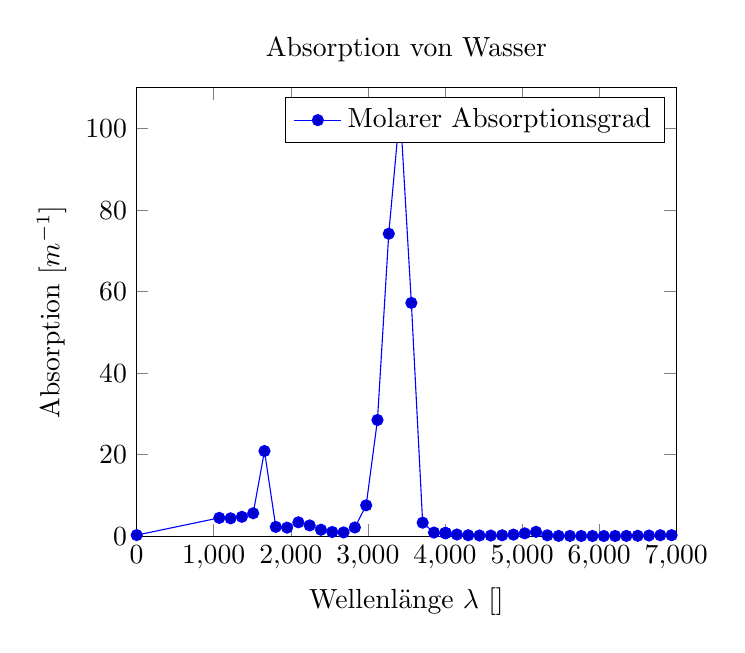
\begin{tikzpicture}
    \centering
    \begin{axis}[
        title={Absorption von Wasser},
        xlabel={Wellenlänge $\lambda$ [\SI{}{\micro\metre}]},
        ylabel={Absorption [$m^{-1}$]},
        xmin=0, xmax=7000,
        ymin=0, ymax=110
    ]

    \addplot table {
        15000.580078125	3.5881996154785156e-05
        14854.016568165016	3.546476364135742e-05
        14707.453058205034	3.7789344787597656e-05
        14560.88954824505	4.011392593383789e-05
        14414.326038285068	4.500150680541992e-05
        14267.762528325084	5.245208740234375e-05
        14121.1990183651	6.222724914550781e-05
        13974.635508405117	8.213520050048828e-05
        13828.071998445133	0.00011175870895385742
        13681.508488485151	0.0001608133316040039
        13534.944978525167	0.00021374225616455078
        13388.381468565183	0.00022125244140625
        13241.817958605201	0.00022369623184204102
        13095.254448645217	0.00022369623184204102
        12948.690938685235	0.0002187490463256836
        12802.12742872525	0.00020694732666015625
        12655.563918765267	0.00019288063049316406
        12509.000408805285	0.00017684698104858398
        12362.4368988453	0.00017023086547851562
        12215.873388885317	0.00017946958541870117
        12069.309878925334	0.00023496150970458984
        11922.74636896535	0.00030434131622314453
        11776.182859005368	0.0003287792205810547
        11629.619349045384	0.0003460049629211426
        11483.055839085402	0.00037747621536254883
        11336.492329125418	0.0004226565361022949
        11189.928819165434	0.00047469139099121094
        11043.365309205452	0.0005293488502502441
        10896.801799245468	0.0006363987922668457
        10750.238289285484	0.0009674429893493652
        10603.674779325502	0.0016300082206726074
        10457.11126936552	0.0031131505966186523
        10310.547759405534	0.0037643909454345703
        10163.984249445552	0.0037239789962768555
        10017.42073948557	0.003260016441345215
        9870.857229525585	0.0026285648345947266
        9724.293719565601	0.0019841790199279785
        9577.73020960562	0.0014564990997314453
        9431.166699645635	0.0011605024337768555
        9284.603189685651	0.0011202692985534668
        9138.039679725669	0.0013459324836730957
        8991.476169765687	0.0017933845520019531
        8844.912659805701	0.002694845199584961
        8698.349149845719	0.0075002312660217285
        8551.785639885737	0.009478449821472168
        8405.222129925753	0.009922683238983154
        8258.658619965769	0.009851276874542236
        8112.0951100057855	0.009245872497558594
        7965.531600045802	0.008631110191345215
        7818.968090085819	0.008717894554138184
        7672.404580125836	0.010782182216644287
        7525.841070165852	0.016894102096557617
        7379.277560205869	0.026682019233703613
        7232.714050245886	0.050036609172821045
        7086.150540285903	0.18809884786605835
        6939.58703032592	0.252522349357605
        6793.023520365936	0.23750674724578857
        6646.460010405954	0.16313821077346802
        6499.89650044597	0.10830909013748169
        6353.332990485986	0.07362180948257446
        6206.7694805260035	0.056888043880462646
        6060.2059705660195	0.048353731632232666
        5913.642460606037	0.04578763246536255
        5767.078950646053	0.051561713218688965
        5620.515440686069	0.07034063339233398
        5473.951930726087	0.07269662618637085
        5327.388420766103	0.21629035472869873
        5180.824910806121	1.0725154876708984
        5034.261400846137	0.6989980936050415
        4887.697890886153	0.3837106227874756
        4741.134380926171	0.22514116764068604
        4594.570870966187	0.1640833616256714
        4448.0073610062045	0.1647963523864746
        4301.4438510462205	0.23776960372924805
        4154.8803410862365	0.4119962453842163
        4008.3168311262543	0.7652896642684937
        4007.3525975080956	0.7661719918251038
        4006.388363889939	0.7670530080795288
        4005.42413027178	0.7679343223571777
        4004.459896653623	0.7688151001930237
        4003.4956630354645	0.7696946859359741
        3856.9321530754823	0.8924610614776611
        3710.3686431154983	3.316239356994629
        3563.8051331555143	57.23850631713867
        3417.241623195532	104.81078338623047
        3270.678113235548	74.21890258789062
        3124.114603275566	28.51203727722168
        2977.551093315582	7.574705123901367
        2830.987583355598	2.14326810836792
        2684.424073395616	0.9271015524864197
        2537.860563435632	1.03183913230896
        2391.2970534756496	1.5820685625076294
        2244.7335435156656	2.6478028297424316
        2098.1700335556816	3.4110329151153564
        1951.6065235956994	2.100344181060791
        1805.0430136357154	2.284926652908325
        1658.4795036757332	20.891077041625977
        1511.9159937157492	5.626224517822266
        1365.3524837557652	4.752559661865234
        1218.788973795783	4.38520622253418
        1072.225463835799	4.495628356933594
        0.9619140625	0.2680339813232422
    };
    \legend{
        Molarer Absorptionsgrad % EM
    }
    \end{axis}
\end{tikzpicture}